
This section explores how core fusion affects the performance of the SD-VBS benchmarks.
We first perform a phase analysis, followed by a study of the IPC variation for static core fusion.
We then motivate the use of dynamic core fusion using the information gathered.

\subsection{Phase Detection}
Figure~\ref{fig:sxt} presents the IPC performance through time for all the benchmarks when using a logical core (LC) composed of 16 cores.
The IPC is calculated for each time tick, which is set at interval of 640 blocks committed.
The IPC varies a lot for some of the benchmarks such as \bm{Disparity} or \bm{Localization} where we expect dynamic fusion to be especially good.
For other, such as \bm{Multi\_NCut}, the execution is dominated by a single long phase with constant IPC, which will clearly show no benefit from using dynamic fusion.

To better understand how dynamic core fusion improves performance, either by improving speedup or reducing energy, we first study how each benchmark features different phases during their execution.
For every benchmark we regroup the IPC results of 16,8,4,2,1 fused cores and use kMeans clustering to determine phases.
This process is only done for the purpose of exploring this set of benchmarks.
Intervals that exhibit similar IPC values when run on different core counts are classified in the same cluster.
In order to find the correct number of clusters we plot the Sum of Square Errors (SSE) for a given cluster size from 1 to 15 and determine the optimal cluster to be in the elbow in the plot~\cite{everitCluster2001}.

\vspace{5mm}
Figure~\ref{fig:clust} shows us the optimal number of clusters for each benchmark and the frequency of each cluster.
The data can be corroborated with the information found in Figure~\ref{fig:sxt}.
For example, benchmarks \bm{MSER} and \bm{Multi\_NCut} feature two phases, with one dominating phase.
This means that it will be impossible to obtain any kind of performance improvements through dynamic reconfiguration.
For all the other benchmarks, they each have at least two dominant phases.
Since each phase is a cluster of similar IPC values, having two or more clusters will result in a higher chance of benefiting from dynamic core fusion.


\begin{figure*}[t]
    \centering
    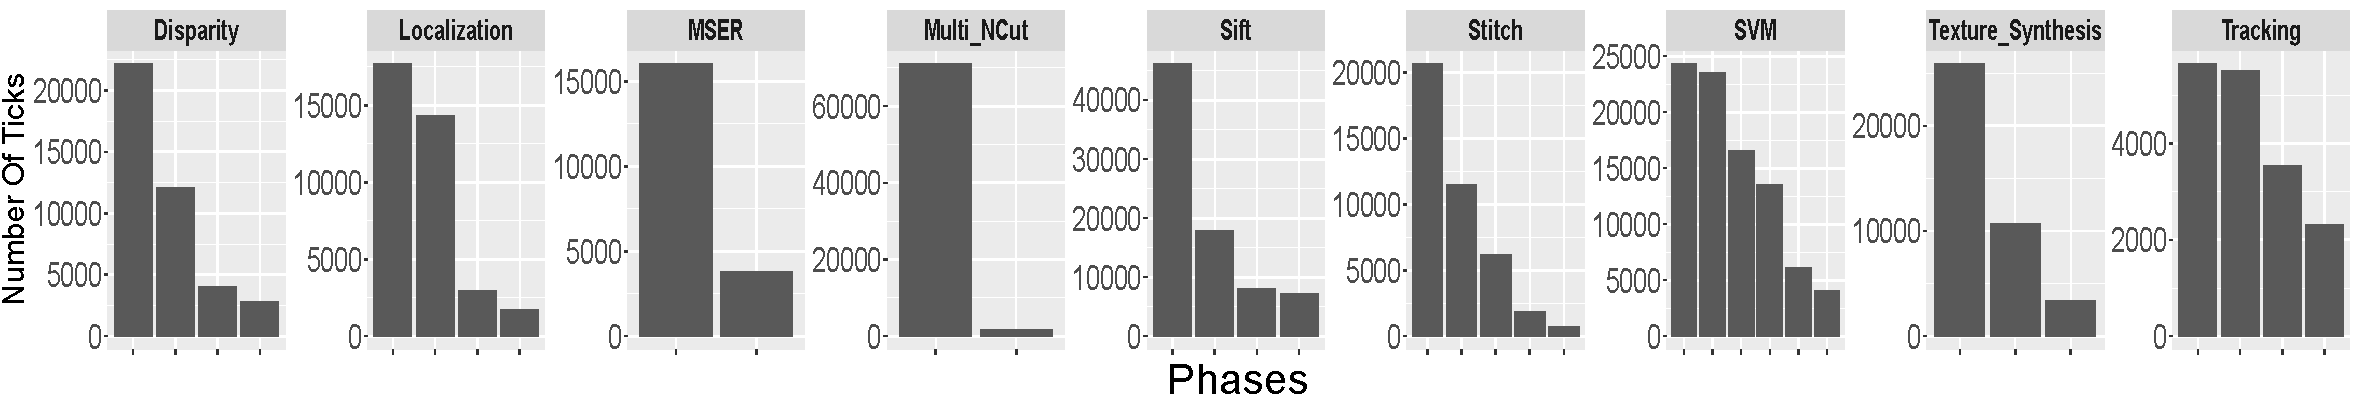
\includegraphics[width=1\textwidth]{cases-paper/graphics/Exploration/clusters2.pdf}
        \vspace*{-7mm}
    \caption{Number of phases determined for each benchmark using kMeans clustering and their distribution.}
    \label{fig:clust}
\label{some example}
\end{figure*}

\begin{figure*}[t]
    \centering
    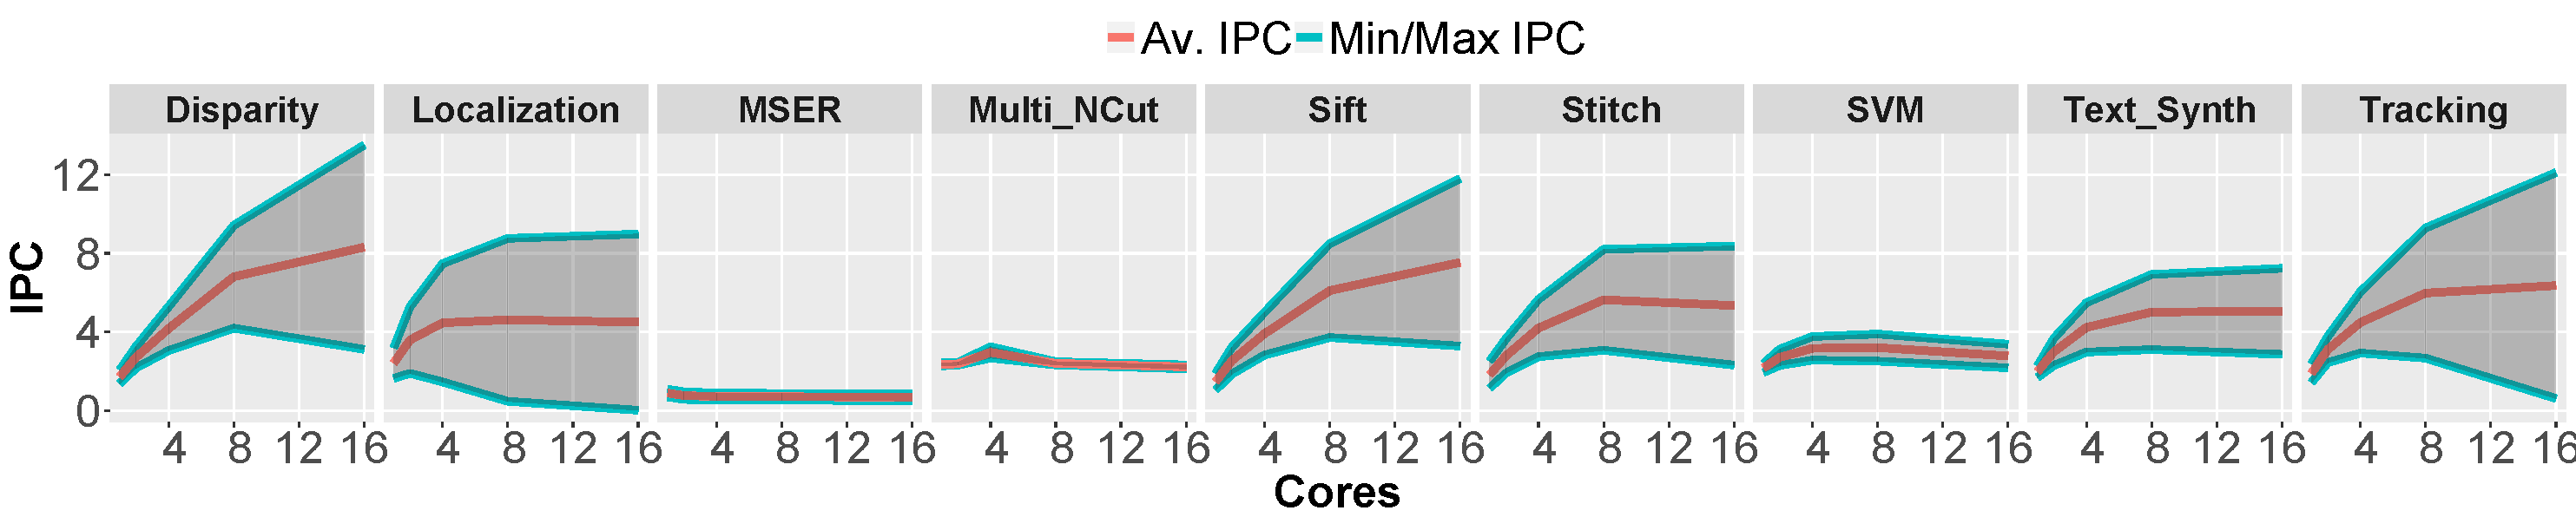
\includegraphics[width=1\textwidth]{cases-paper/graphics/Exploration/stddev.pdf}
        \vspace*{-7mm}
    \caption{Comparing average, smallest and greatest IPC for each SD-VBS benchmark using logical-core size of 16.}
    \label{fig:stddev}
\vspace{5mm}
\end{figure*}
\subsection{Static Core Fusion Exploration}

Figure~\ref{fig:stddev} shows how the average Instructions Per Cycle (IPC) changes as we increase the size of a LC, going in powers of 2 from 1 to 16 fused cores.
We see that, for most benchmarks, fusing more cores provides an increase in IPC performance.
Benchmarks \bm{Disparity}, \bm{Localization}, \bm{Sift}, \bm{Stitch}, \bm{Texture Synthesis} and \bm{Tracking} all at least observe a speedup of 2x when using core fusion.

However increasing the size of a LC is not always beneficial as can be seen in benchmarks \bm{Localization}, \bm{MSER}, \bm{Multi\_NCut}, \bm{Stich}, and \bm{SVM}.
For benchmarks \bm{Localization} and \bm{Stitch} the performance increases when fusing up to 8 cores, where-as \bm{MSER} and \bm{Multi\_NCut} never benefit from core fusion. 
Referring back to Figures~\ref{fig:sxt} and~\ref{fig:clust}, we can see that \bm{MSER} and \bm{Multi\_NCut} feature one dominating long phase, both performing poorly.
This explains the lack of scaling for these two benchmarks.

Figure~\ref{fig:stddev} also shows the standard deviation of the IPC for each given LC size represented by the grayed out areas.
For example, running the \bm{Disparity} benchmark on a LC of 16 cores, we have an average IPC of 8.3 with a standard deviation of 5.2.
The standard deviation for 16 cores shows that the performance can drop down to 2.5.
An IPC of 2.5 when using 16 cores is very inefficient as this represents 0.1 of an instruction per cycle for each core.
We can observe that when using a LC of size 4 for the \bm{Disparity} benchmark we achieve an average of 4.1 with a standard deviation of 1.2.
Thus, if the logical-core could change size, there is a possibility that we could reduce the overall energy consumption of the system by switching from 16 to 4.

Overall, most benchmarks that benefit from large logical-cores will also be met with important standard deviations of IPC performance.
The high standard deviation is evidence of performance phases found in each application which are likely to benefit from dynamic adaptation.
